%! Author = TiagoRG
%! GitHub = https://github.com/TiagoRG

\chapter{Análise e Discussão}
\label{ch:analise-discussao}
{
%%%
% Conteúdo da Análise e Discussão aqui

\section{Parte A}
\label{sec:analise-discussao-parte1}

\subsection{Análise}
\label{subsec:analise-discussao-parte1-analise}

\subsubsection{Distância}
\label{subsec:analise-discussao-parte1-distancia}

Esta distância é 10cm e será constante para todos os lançamentos sendo ela a distância entre os dois sensores de movimento. O erro associado a esta medição é de 1mm.

\subsubsection{Tempo}
\label{subsec:analise-discussao-parte1-tempo}

O tempo é medido pelo sistema de controlo dos sensores e é medido em segundo. O erro associado a esta medição é de 0.0001s. Este tempo é em média 0.04447s. A variação máxima do tempo é 0.0005s.

\subsubsection{Velocidade}
\label{subsec:analise-discussao-parte1-velocidade}

Para calcular a velocidade utilizamos a seguinte fórmula:

\begin{equation}
    v = \frac{d}{t}
\end{equation}

O erro associado a esta medição é de 0.0001m/s. A velocidade média é 2.249m/s. A variação máxima da velocidade é 0.04778m/s.

\subsection{Discussão}
\label{subsec:analise-discussao-parte1-discussao}

Tendo em conta as medições anteriores da distância e do tempo, verifica-se que a distância foi constante e a variação do tempo bastante baixa (variação máxima de 0.0005s) o que implica uma exatidão alta nos valores da velocidade calculados (exatidão de 97.9\%).\bigskip

Entre os possíveis motivos para a variação nos valores medidos de tempo podem se mencionar:
\begin{itemize}
    \item A falta de consistência da força da mola;
    \item A forma como a pessoa que dispara pode não o fazer exatamente da mesma forma em todos os disparos.
\end{itemize}

\pagebreak

\section{Parte B}
\label{sec:analise-discussao-parte2}

\subsection{Análise}
\label{subsec:analise-discussao-parte2-analise}

\subsubsection{Altura}
\label{subsec:analise-discussao-parte2-altura}

O valor da altura será constante e será medido desde o nível do alvo até ao ponto de lançamento verticalmente. No caso desta experiência, a altura medida foi 26cm.

\subsubsection{Ângulo}
\label{subsec:analise-discussao-parte2-angulo}

Este ângulo varia de lançamento para lançamento, sendo medido utilizando as marcações do lançador. O erro associado a esta medição é de 0.5º. Os valores usados foram 30º, 34º, 38º, 40º e 43º.

\subsubsection{Alcance}
\label{subsec:analise-discussao-parte2-alcance}

A figura \ref{fig:parte2-chart} representa o alcance em função do ângulo. No eixo $x$ temos o ângulo de lançamento enquanto que no eixo $y$ temos o alcance médio de cada ângulo.

\begin{figure}[ht]
    \centering
    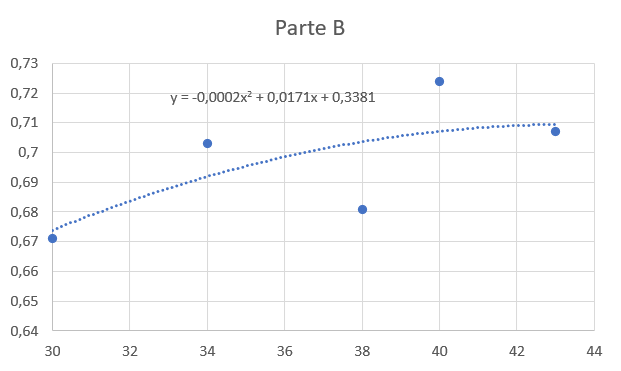
\includegraphics[width=0.6\textwidth]{images/parte2chart.png}
    \caption{Gráfico do alcance em função do ângulo}
    \label{fig:parte2-chart}
\end{figure}

\subsection{Discussão}
\label{subsec:analise-discussao-parte2-discussao}

Tendo em conta os valores obtidos, verifica-se uma maior discrepância entre esses mesmos valores, especialmente para os três primeiros ângulos usados (30º, 34º e 38º) com variações de 0.051, 0.046 e 0.046, respetivamente.\bigskip

Nesta experiência, estas variações podem se dever a diversos fatores, como por exemplo:
\begin{itemize}
    \item A falta de consistência da força da mola;
    \item A forma como a pessoa que dispara pode não o fazer exatamente da mesma forma em todos os disparos;
    \item A resistência do ar;
    \item As marcas existentes no alvo que podem causar confusão à pessoa que as vai verificar;
    \item A pouca estabilidade do alvo;
    \item Pequenas variações na forma de medição do alcance.
\end{itemize}\bigskip

Para calcular o ângulo para o qual o alcance é máximo, é necessário calcular a derivada da função do alcance em função do ângulo e igualar a zero. A função do alcance em função do ângulo foi obtida utilizando o software Microsoft Excel que aproximou uma função polinomial de segundo grau aos pontos respetivos aos nossos valores. A equação obtida foi, tal como se pode ver no gráfico da figura \ref{fig:parte2-chart}:

\begin{equation}
    y = -0.0002x^2 + 0.0171x + 0.3381
\end{equation}

A derivada desta função em $x$ será:

\begin{equation}
    y' = -0.0004x + 0.0171
\end{equation}\\
Por sua vez, esta será igual a 0 quando $x = 42.75$º.\bigskip

A altura de lançamento usada foi a mesma para todos os disparos de todos os ângulos o que implica que, baseado na experimentação, o ângulo para o qual se obtém maior alcance será $42.75$º.

\pagebreak

\section{Parte C}
\label{sec:analise-discussao-parte3}

\subsection{Análise}
\label{subsec:analise-discussao-parte3-analise}

\subsubsection{Comprimento do pêndulo}
\label{subsec:analise-discussao-parte3-comprimento}

Distância entre o ponto de suspensão e extremidade do centro. Este valor é obtido por medição direta com o erro associado de 1mm. O valor obtido foi de 24.4cm.

\subsubsection{Massas}
\label{subsec:analise-discussao-parte3-massas}

As massas são obtidas por medição direta com o erro associado de 0.1g. Os valores obtidos foram 237.2g para o pêndulo e 66.5g para o projétil.

\subsubsection{Ângulo}
\label{subsec:analise-discussao-parte3-angulo}

Este é o ângulo máximo descrito pelo movimento do pêndulo. O erro associado a esta medição é de 0.1º. O valor médio foi 17º.

\subsubsection{Altura}
\label{subsec:analise-discussao-parte3-altura}

Este é o valor da altura máxima atingida pelo projétil, que é registada no ponto de maior ângulo. Pode ser calculada a partir da seguinte fórmula:

\begin{equation}
    h = L(1 - \cos(\theta))
\end{equation}

O valor médio obtido foi 10.66mm.

\subsubsection{Velocidade}
\label{subsec:analise-discussao-parte3-velocidade}

Este é o valor da velocidade inicial do projétil. Pode ser calculada a partir da seguinte fórmula:

\begin{equation}
    v = \left| \frac{m_{projetil}~+~m_{pendulo}}{m_{projetil}} * \sqrt{2*g*h} \right|~~~~~(SI)
    \label{eq:parte3-velocidade-inicial}
\end{equation}

Onde $g$ é a aceleração gravítica e $h$ é a altura máxima atingida pelo projétil (calculada anteriormente).

\subsection{Discussão}
\label{subsec:analise-discussao-parte3-discussao}

Tendo em conta os valores obtidos, verifica-se uma amplitude de 1º. Esta variação pode se dever a diversos fatores, como por exemplo:

\begin{itemize}
    \item A falta de consistência da força da mola;
    \item A forma como a pessoa que dispara pode não o fazer exatamente da mesma forma em todos os disparos;
    \item Incerteza associada ao instrumento de medição;
    \item O atrito do pêndulo com o suporte.
\end{itemize}

Usando a fórmula \ref{eq:parte3-velocidade-inicial} obtém-se para cada ângulo diferentes valores de velocidade inicial, sendo o valor da velocidade média 2.0879m/s. Este resultado deverá ser semelhante ao obtido da Parte A (secção \ref{subsec:analise-discussao-parte1-velocidade}), que ao comparar verifica-se uma diferença de 0.1611m/s.

%%%
}
